%%%%%%%%%%%%%%%%%%%%%%%%%%%%%%%%%%%%%%%%%%%%%%%%%%%%%%%%%%%%%%%%%%%%%%%%
%    INSTITUTE OF PHYSICS PUBLISHING                                   %
%                                                                      %
%   `Preparing an article for publication in an Institute of Physics   %
%    Publishing journal using LaTeX'                                   %
%                                                                      %
%    LaTeX source code `ioplau2e.tex' used to generate `author         %
%    guidelines', the documentation explaining and demonstrating use   %
%    of the Institute of Physics Publishing LaTeX preprint files       %
%    `iopart.cls, iopart12.clo and iopart10.clo'.                      %
%                                                                      %
%    `ioplau2e.tex' itself uses LaTeX with `iopart.cls'                %
%                                                                      %
%%%%%%%%%%%%%%%%%%%%%%%%%%%%%%%%%%
%
%
% First we have a character check
%
% ! exclamation mark    " double quote  
% # hash                ` opening quote (grave)
% & ampersand           ' closing quote (acute)
% $ dollar              % percent       
% ( open parenthesis    ) close paren.  
% - hyphen              = equals sign
% | vertical bar        ~ tilde         
% @ at sign             _ underscore
% { open curly brace    } close curly   
% [ open square         ] close square bracket
% + plus sign           ; semi-colon    
% * asterisk            : colon
% < open angle bracket  > close angle   
% , comma               . full stop
% ? question mark       / forward slash 
% \ backslash           ^ circumflex
%
% ABCDEFGHIJKLMNOPQRSTUVWXYZ 
% abcdefghijklmnopqrstuvwxyz 
% 1234567890
%
%%%%%%%%%%%%%%%%%%%%%%%%%%%%%%%%%%%%%%%%%%%%%%%%%%%%%%%%%%%%%%%%%%%
%
\documentclass[12pt]{iopart}
\bibliographystyle{iopart-num_custom}
\usepackage{xcolor}
\usepackage{pifont}
\usepackage{comment}
\usepackage{acronym}
%\usepackage{subcaptncluon}
\usepackage{tikz}
\usetikzlibrary{shapes.geometric, arrows, calc}
\expandafter\let\csname equation*\endcsname\relax 
\expandafter\let\csname endequation*\endcsname\relax 
\usepackage{amsmath}
\usepackage{amssymb}
\usepackage{hyperref}
\newcommand{\gguide}{{\it Preparing graphics for IOP Publishing journals}}
%Uncomment next line if AMS fonts required
%\usepackage{iopams}  
\newcommand{\jordan}[1]{\textbf{\textcolor{red}{JORDAN: #1}}}
\newcommand{\siong}[1]{\textbf{\textcolor{blue}{SIONG: #1}}}
\newcommand{\chris}[1]{\textbf{\textcolor{green}{CHRIS: #1}}}
\newcommand{\michael}[1]{\textbf{\textcolor{orange}{MICHAEL: #1}}}
\newcommand{\dcc}{LIGO-PXXXXXXX}
\input{tag.tex}
\begin{document}

\title{Generalised gravitational burst generation with Generative Adversarial Networks}

\author{J. McGinn, C. Messenger, I.S. Heng}

\address{University of Glasgow, Physics \& Astronomy Department, Glasgow G12 8QQ, UK}
%\ead{jordan.mcginn@glasgow.ac.uk}
\vspace{10pt}
\begin{indented}
\item[]\commitDATE\\\mbox{\small \commitID}\\\mbox{\dcc}
\end{indented}

\begin{abstract}
The next generation of Gravitational wave detectors will accelerate the number
of gravitational wave detection's such that we can gain new in site into the
physics behind the sources causing the phenomena. Numerical simulations and
matched filtering are the standard for detecting gravitational waves for know
sources such as binary-black hole mergers. Other sources of gravitational waves
that remain elusive to standard modelling techniques and are expected to be
detectable, however, there must be a way to characterise them in order to build
a model template. Here we construct a unmodeled burst generation scheme using
Generative adversarial networks - a powerful class of machine learning.
\end{abstract}

%
% Uncomment for keywords
%\vspace{2pc}
%\noindent{\it Keywords}: XXXXXX, YYYYYYYY, ZZZZZZZZZ
%
% Uncomment for Submitted to journal title message
%\submitto{\JPA}
%
% Uncomment if a separate title page is required
%\maketitle
% 
% For two-column output uncomment the next line and choose [10pt] rather than [12pt] in the \documentclass declaration
%\ioptwocol
%

\acrodef{GW}[GW]{gravitational wave}
\acrodef{GAN}[GAN]{generative adversarial networks}
\acrodef{CGAN}[CGAN]{conditional generative adversarial networks}
\acrodef{ACGAN}[ACGAN]{auxilliary conditional generative adversarial networks}
\acrodef{BBH}[BBH]{binary black hole}


\section{Introduction}
\begin{comment}
\begin{itemize}
\item Need to introduce GWs - the current state of the field e.g. detections
and LVC papers \ding{51}
\item Introduce burst searches - what's the point of burst searches \ding{51} - lots of references 
\item Discuss the family of burst waveforms currently used and why - not in detail, just
an introduction \ding{51}
\item Introduce ML techniques in GWs \ding{51} - lots of references
\item What this paper does on GANs in 1 paragraph \ding{51}
\item Describe the structure of the paper 
\end{itemize}
\end{comment}

% introduce \ac{GW} astrophsyics
%
\ac{GW} astronomy is now an established field, starting with the first
detection of a binary black hole merger \cite{Abbott2016} in September 2015.
Following this, the first and second observations runs (O1 and O2) of Advanced
LIGO and Advanced Virgo~\chris{need refs for the detectors, see here
https://pnp.ligo.org/ppcomm/standard\_references.html} reported several more
mergers \cite{Abbott2016a, Abbott2017, Abbott2017a, Abbott2017b}. On August
2017 a binary neutron star merger was observed alongside its electromagnetic
counterpart for the first time, giving rise to multimessenger gravitational
wave astronomy. 

% introduce burst searches
%
GW bursts are transient signals of typically short duration ($<$ 1s) whose
waveforms are not accurately modelled or are complex to re-produce.
Astrophysical sources for such transients include: Core collapse supernova,
Neutron star instabilities, Fallback accretion onto a neutron star, Non
axisymetric deformation in magnetars, Pulsar glitches and Neutron star
post-mergers.  As \ac{GW} bursts are un-modelled they are not sensitive to
template based detection schemes~\chris{OK, but logically dodgy. You make it
sound like we could use a template scheme but it would be insensitive. The
point is that we don't have templates in the first place.} such as
matched-filtering \cite{Owen1998}, instead, detection involves distinguishing
the signal from detector noise. This is only possible if the detector noise is
well characterised and the candidate signal can be differentiated from
systematic or environmental glitches. As such, \ac{GW} burst searches rely on
an astrophysical burst signature appearing in multiple detectors~\chris{at
similar times?}.  

% Discuss the family of burst waveforms currently used and why - not in detail, just
% an introduction 
%
Many \ac{GW} burst algorithms \cite{Klimenko_2008, Aso_2008}~\chris{many? needs
more than 2 refs for many.} are tested and tuned using model waveforms that may
or may not have astrophysical significance but have easy to define parameters
and share characteristics of real bursts that is enough to simulate coincident
non-stationary deviations~\chris{fancy sounding but I'm not sure what
non-stationary deviations means.} between detectors. Such waveforms may have
long-duration, short bandwidth (ringdowns), long-duration, large bandwidth
(inspirals) and many algorithms make use of sine-Gaussians: a Gaussian
modulated sine wave that is characterised by it's central frequency and narrow
bandwidth.~\chris{not the time to try to describe the types of burst waveforms.
Also, be careful with satying things like ringdowns have narrow bandwidth. I
know we specify a single frequency but becuase of the short duration, the
signal is broad band. Look at the FFT} This makes it a great tool for
diagnosing LIGOs sensitivity to frequency.~\chris{strange unfinished sentence.} 

% Introduce ML techniques in GWs
%
\chris{Introduce ML techniques in GWs}

% What this paper does on GANs in 1 paragraph
%
\chris{What this paper does on GANs in 1 paragraph}

% the point of the paper
%
\chris{describe the structure of the paper}
We aim to explore the use of machine learning in generating and interpreting
these mock \ac{GW} burst signals. Neural networks have shown to replicate the
sensitivities of matched filtering in \ac{GW} detection \cite{Gabbard2017} and rapid
parameter estimation \cite{gabbard2019bayesian}, however these methods have
primarily been focused on binary black hole signals and have not yet expanded
to burst examples.~\chris{OK, thanks for the referdndes but you should probably
have more refs to other ML GW papers. I think you should dedicate at least one
paragrpah to GW ML efforts. The final paragrapgh of the section should
introduce the paper structure. The penultimate paragraph should expain what the
point of this paper is - in non technical terms. This is all outlined in the
bullet points (hidden) at the start of this section.} 

%%%%%%%%%%%%%%%%%%%%%%%%%%%%%%%%%%%%%%%%%%%%%%%%%%%%%%%%%%%%%%%%%%%%%%%%%%%%%%
\section{Generative Adversarial Networks}
%%%%%%%%%%%%%%%%%%%%%%%%%%%%%%%%%%%%%%%%%%%%%%%%%%%%%%%%%%%%%%%%%%%%%%%%%%%%%%

\begin{comment}
\begin{itemize}
\item Describe GANs in detail but really focus on the fact that the reader is a
GW data analyst - not a computer scientist \ding{51}
\item A diagram would be very useful \ding{51}
\item Do not discuss our specific case here - just stay general \ding{51}
\item A subsection on the specific advanced flavour of GAN that you are using
here - motivate this choice. \ding{51}
\end{itemize}
\end{comment}

% introduce GANs
%
A subset of deep learning that has seen fruitful development in recent years
\cite{Goodfellow2014} is \acp{GAN}. These unsupervised algorithms learn
patterns in a given training data set using an adversarial process. The
generations from \acp{GAN} are state-of-the-art in fields such as high quality image
fidelity \cite{brock2018large,karras2019analyzing}, text-to-image translation
\cite{reed2016generative} and video prediction \cite{liang2017dual} as well as
time series generations \cite{esteban2017realvalued}. 

% How a GAN works
%
\acp{GAN} train two competing neural networks, consisting of a discriminator
that is set up to distinguish between real and fake data and a generator that
produces synthetic reproductions of the real data. The generator performs a
mapping from an input noise vector $\mathbf{z}$ to its representation of the
data and the discriminator maps its input $\mathbf{x}$ to a probability that
the input came form either the training data or generator.  During training,
the discriminator is given a batch of samples that contains one half real data
and one half fake data which it then makes predictions on. The loss for the
discriminator is calculated by comparing its predictions to the labelled data
through the binary cross-entropy function. The training process of a \ac{GAN}
alternatively updates the weights~\chris{too much knowledge assumed - what are
weights, they haven't been defined} of the discriminator and generator based on
information on its competitors loss function. This loss of discriminator is
used to update the weights of the generator to produce more realistic samples
of the input distribution, the loss of G~\chris{what is G?} encourages the
discriminator to update its classification abilities. Both networks compete in
a minimax game~\chris{what is a minimax game? references?} which the generator
is trying to minimise and the discriminator is trying to
maximise:~\chris{nicely written, however, it needs an extra 25\% explanation
for people not familar with ML or GANs in particular. Try to spell things out
more. Also refer to Fig 1 somewhere in this section.}
%
\begin{equation}
\mathop{\text{min}}_{G}  \mathop{\text{max}}_{D} V(D,G) = \mathbb{E}_{\mathbf{x} \sim p_{\text{r}}(\mathbf{x})} [\text{log} D(\mathbf{x})] \\ + \mathbb{E}_{\mathbf{z} \sim p_{\text{z}}(\mathbf{z})} [\text{log}(1-D(G(\mathbf{z})))]
\label{equation:GANloss}
\end{equation}
%
~\chris{In line with explanding the explanation a bit more, really take the time
to state what controls the functions and also deine ALL mathematical variables.
What are $D, G, V\ldots$ Why are you taking the logs? What situation so you
start with? What do you end up with? This is a nice start but beef it up.}

\subsection{Auxiliary conditional GANs}

% describing the problems with GANs 
%
In theory, the adversarial process will eventually lead to the local Nash
equilibrium \cite{Nash1950} whereby both neural networks are trained
optimally~\chris{this statement and this paragraph should be stated in the
previous section}.  In practice, however, \acp{GAN} are notoriously difficult
to train. Such difficulties include: Non-convergence, where the model
parameters~\chris{you haven't stated what the model parameters are yet}
oscillate and the loss~\chris{the reader soes not know what the loss is and
what the point of it is} never converges, mode collapse where G produces a
limited diversity of samples~\chris{samples of what?}, and diminishing
gradients when applying gradient descent to a non-continuous
function~\chris{not sure about what non-continuous means here but in general
you are bringing in too many concepts without explanation e.g., gradient
descent, why is that relevant? the reader does not know.}. 

% introduce CGANs and ACGANs
%
To overcome some of these difficulties, a conditional variant of \acp{GAN}
named \acp{CGAN}~\cite{cgan} adds structure to the latent space~\chris{what is
the latent space - you called it an input noise vector before} by providing the
generator with a class or attribute label. The generator learns to segment the
latent space by clustering distributions which have similar properties, making
a point in latent space conditional on a class~\chris{are we sure about this?
all classes share the same latent space and I don't think that the space gets
segmented into areas corresponding to different classes - I do think that it
gets broken down into spaces with different intrinsic physical properties e.g.,
high frequency, long duration, etc...}. This idea was extended further with
\acp{ACGAN}~\cite{odena2016conditional} that require the discriminator to
output a probability of data belonging to each class. A pictorial
representation on the differences between these approaches is shown in
Fig.~\ref{fig:gan_comparison}. 

\begin{figure}
    \centering
        %\documentclass{article}
%\usepackage{comment}
%\usepackage{tikz}
%\usetikzlibrary{shapes.geometric, arrows, calc}

%\begin{document}
    
\begin{tikzpicture}[node distance=2cm]

\tikzstyle{zinput} = [rectangle, rounded corners, text centered, draw=black]%, fill=red!30]
\tikzstyle{generator} = [rectangle, rounded corners, text centered, draw=black]%, fill=red!30]
\tikzstyle{X real} = [rectangle, rounded corners, text centered, draw=black]%, fill=red!30]
\tikzstyle{X fake} = [rectangle, rounded corners, text centered, draw=black]%, fill=red!30]
\tikzstyle{X real} = [rectangle, rounded corners, text centered, draw=black]%, fill=red!30]
\tikzstyle{discriminator} = [rectangle, rounded corners, text centered, draw=black]%, fill=red!30]
\tikzstyle{real/fake} = [rectangle, rounded corners, text centered, draw=black]%, fill=red!30]

\tikzstyle{arrow} = [thick,->,>=stealth]

\node (r) [X real] {\textbf{X} real};
\node (f) [X fake, right of = r] {\textbf{X} fake};
\node (G) [generator,above of = f, scale = 2] {\textbf{G}};
\node (z) [zinput] [zinput, above of = G] {\textbf{z} (noise)};
\node (D) [discriminator, below of = f, xshift = -1cm, scale = 2] {\textbf{D}};
\node (rf) [real/fake, below of = D] {real/fake};

\draw [arrow] (z) -- (G);
\draw [arrow] (G) -- (f);
\draw [arrow] (r) edge[out=270,in=90] (D);
\draw [arrow] (f) edge[out=270,in=90] (D);
\draw [arrow] (D) -- (rf);

\end{tikzpicture}
%\end{document}
%     without .tex extension
        \begin{tikzpicture}[node distance=2cm]

\tikzstyle{zinput} = [rectangle, rounded corners, text centered, draw=black]%, fill=red!30]
\tikzstyle{generator} = [rectangle, rounded corners, text centered, draw=black]%, fill=red!30]
\tikzstyle{X real} = [rectangle, rounded corners, text centered, draw=black]%, fill=red!30]
\tikzstyle{X fake} = [rectangle, rounded corners, text centered, draw=black]%, fill=red!30]
\tikzstyle{X real} = [rectangle, rounded corners, text centered, draw=black]%, fill=red!30]
\tikzstyle{discriminator} = [rectangle, rounded corners, text centered, draw=black]%, fill=red!30]
\tikzstyle{real/fake} = [rectangle, rounded corners, text centered, draw=black]%, fill=red!30]
\tikzstyle{coutput} = [rectangle, rounded corners, text centered, draw=black]%, fill=red!30]

\tikzstyle{arrow} = [thick,->,>=stealth]

\node (r) [X real] {\textbf{X} real};
\node (f) [X fake, right of = r, xshift = 0cm] {\textbf{X} fake};
\node (G) [generator,above of = f, scale = 2] {\textbf{G}};
\node (z) [zinput] [zinput, above of = G, xshift = 1cm] {\textbf{z} (noise)};
\node (c) [coutput, left of = z] {\textbf{c} (class)};
\node (D) [discriminator, below of = f, xshift = -1cm, scale = 2] {\textbf{D}};
\node (rf) [real/fake, below of = D] {real/fake};
%\node (co) [coutput, left of = rf, xshift = -0.5cm] {c = 1, 2, ...};

\draw [arrow] (z) edge[out=270,in=90] (G);
\draw [arrow] (c) edge[out=270,in=90] (D);
\draw [arrow] (c) edge[out=270,in=90] (G);
\draw [arrow] (c) edge[out=270,in=90] (r);
\draw [arrow] (G) -- (f);
\draw [arrow] (r) edge[out=270,in=90] (D);
\draw [arrow] (f) edge[out=270,in=90] (D);
\draw [arrow] (D) edge[out=270,in=90] (rf);
%\draw [arrow] (D) edge[out=270,in=90] (co);

\end{tikzpicture}%     without .tex extension
    \caption{Comparison of the original GAN method and the Auxiliary
Conditional-GAN method. For ACGANs the training data requires a label denoting
its class that is also fed to the generator which then learns to generate
waveforms based on the input label. Additionaly, the discrminator learns to
classify which class the signal belongs to.} \label{fig:gan_comparison}
\end{figure}

\chris{this section is supposed to be on ACGANs but it only mentions them in
the final sentence. Again, like the previous section, a bit more explanation
would be good. Does ths maths change? Could you have a new version of Eq 1 for
CGANs and ACGANs? Also, if would be good to have a statement that you will be
using one of these methods in this paper.}

%%%%%%%%%%%%%%%%%%%%%%%%%%%%%%%%%%%%%%%%%%%%%%%%%%%%%%%%%%%%%%%%%%%%%%%%%%%%%%
\section{Methodology}
%%%%%%%%%%%%%%%%%%%%%%%%%%%%%%%%%%%%%%%%%%%%%%%%%%%%%%%%%%%%%%%%%%%%%%%%%%%%%%

\begin{comment}
\begin{itemize}
\item Need to introduce the scheme you propose to use
\item A paragraph or subsection on the data generation being very clear on all
5 waveform models and the prior parameter space for each \ding{51}
\item A subsection on the design of the network architecture \ding{51}
\item A subsection on the "box" and why we implement it \ding{51}
\item A subsection on the training of the network - give rough timings and rule
of thumb decisions made
\item Do not discuss the results here 
\end{itemize}
\end{comment}

% introduce the training data
%
\ac{GW} burst signals remain an unmodelled phenomenon, as such, current
detection algorithms focus on waveform reconstruction reliant on coincident
signals within multiple detectors~\chris{burst detection algorithms do not need
waveform reconstruction for searches - it is an add on feature.}. We propose a
signal generation scheme utilizing~\chris{utilizing certainly is fancier than
using. Dont go overboard with the language.} \acp{GAN} trained on burst-like
waveforms. The \ac{GAN}~\chris{is it a GAN or is it a CGAN or an ACGAN? Be
clearer} is trained on five signal morphology's spanning a range of prior
parameters. The families are:~\chris{I know they don't all share the same
parameters but it might be sensible to make a table of the prior ranges rather
than haviong it all stated in text.}
%
\begin{itemize}
%
\item Sine-Gaussian:\\
\chris{don't just start things with an equation}		
%
\begin{equation}
\label{eqn:sg}
h(t) = A \exp\bigg[ - \frac{(t-t_{0})^2}{\tau^2} \bigg] \sin (2 \pi f_0 (t-t_0))
\end{equation}	
%		
where $f_0$ is the central frequency that takes values between 30 Hz - 50 Hz.
$\tau$ is the decay parameter chosen to be between 60s$^{-1}$  and 15s$^{-1}$
and the starting epoch chosen between 0.2s - 0.8s. Sine-Gaussian waveforms have
a similar form to those produced by the merger of relatively high mass binary
black holes for which the inspiral phase occurs at frequencies below
ground-based detector sensitivities.
%
\item Ring-down:\\
\chris{don't just start things with an equation}
%
\begin{equation}
h(t) = A \exp \bigg[-\frac{(t-t_0)}{\tau}\bigg]\sin(2 \pi f_0 (t-t_0))
\end{equation}
%		
For ring-down signals the parameters for $f_0, \tau, t_0$ are chosen between;
30 Hz-50Hz, 0.02-0.1 and 0.1s-0.8s respectfully. These signals aim to replicate
the post-merger late stages of binary coalescence.
%
\item White-noise bursts:\\
\chris{where is the waveform equation?}
These signals are produced by inserting samples of random Gaussian noise with
zero mean and a variance of 0.1 at a random point between 0.2s - 0.8s. The
source of this signal type can be attributed to core-collapse
supernova~\chris{is this correct? these waveofms are approximations so best not
to say that they correspond directly to physical phenomena}.
%
\item Gaussian pulse:\\
\chris{where is the waveform equation?}
A simple Gasssian pulse waveform with $t_0$ ranging from 0.2s to 0.8s and
$\tau$ between  100$^{-1}$ and 20$^{-1}$
	
\item Binary black holes (BBH): \\
\ac{BBH} signals are simulated using IMRPhenomD waveform routine from
LALSuite~\chris{references for both the waveofrm and lalsuite} which models the
inspiral, merger and ringdown of a \ac{BBH} waveform. The component masses lie
in the range of [5,70]M$_0$~\chris{not $M_0$ but $M_{\odot}$} with zero spins
and we fix m$_1$ $>$ m$_2$. The mass distribution is approximated by a power
law with index of 1.6 https://arxiv.org/abs/1811.12940~\chris{correct;ly
reference this}. The signals are generated using random right ascensions and
declinations uniform over the sky and the inclinations are drawn from the
cosine of a uniform distribution in the range [-1,1]. The peaks of the
waveforms are set to be within [0.75,0.95]s of the 1s time interval.~\chris{for
all the signal models please check that the prior ranges and distributions are
consistent with the presented results.} 
%
\end{itemize}

\chris{you seem to be missing a description of the antenna patterns and time
delay that you apply to each waveform. It should go here. You should also
include all other technical information like how you normalise the amplitudes
and how you select random sky positions, how the data is represented to the
network (as an image or as channels) how many detectors do you use? etc... }

\begin{figure}
    \centering
    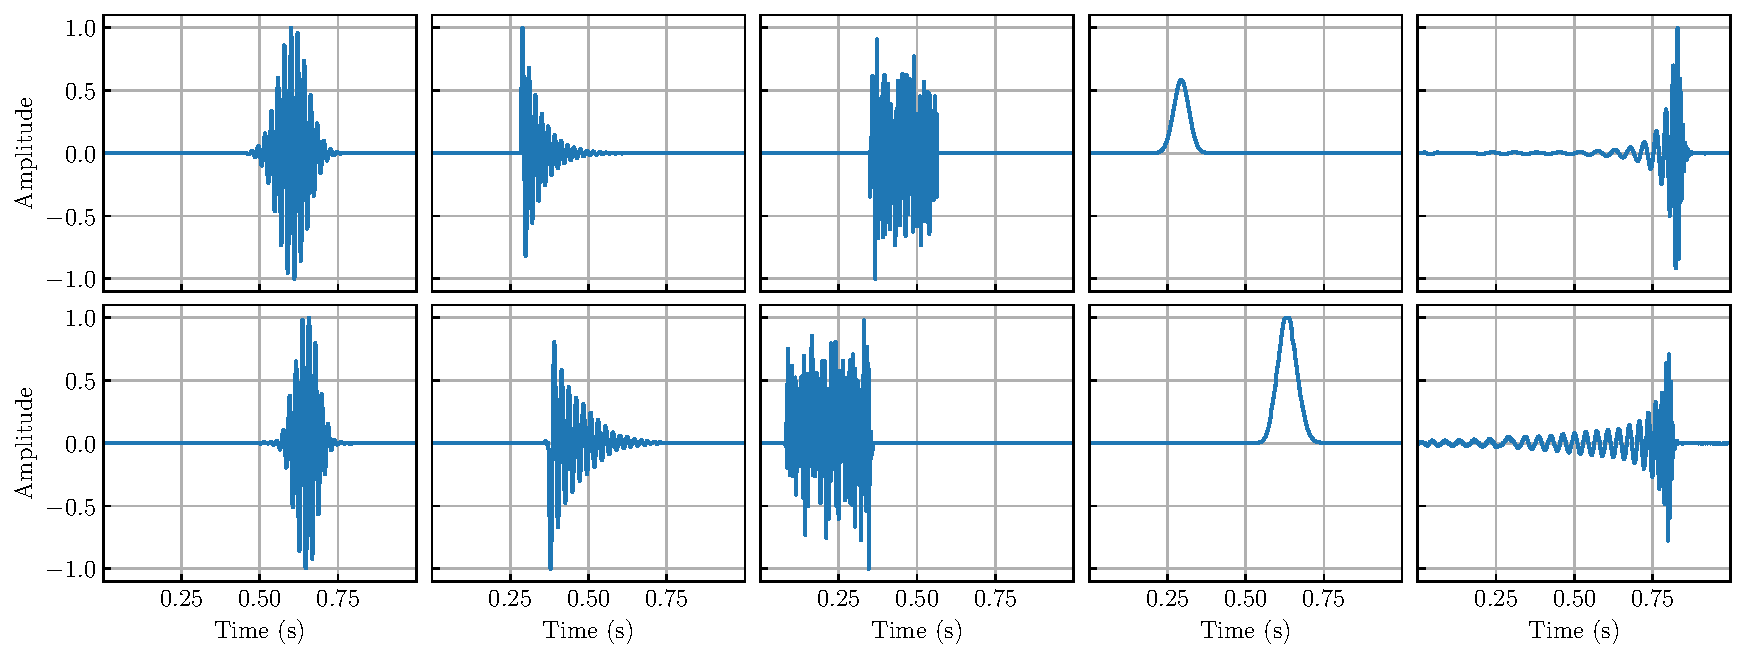
\includegraphics[width=\textwidth]{figures/train_gen.pdf}
    \caption{Examples of simulated \ac{GW} burst signals. Top row shows
examples from the training set. From left to right: Sine-Gaussian, Ringdown,
White-noise burst, Gaussian pulse, Binary black hole merger. The bottom row
shows the conditional generations from the GAN.~\chris{slightly more
explanation. The reader may be concerned that the top and bottom do not look
the same. Should they? They may wonder why is there only one waveform and not
one per detector?} } \label{fig:train} \end{figure}

\subsection{Architecture details}
Extensions to the original GAN method such as  DCGANs \cite{Radford2015} have been widely praised for building a stable GAN architecture. Modern GAN research favours a fully convolution neural network which replace upsampling procedures like maxpooling to strided convolutions. Convolutional neural networks (CNNs) are designed to work with grid-like structures that exhibit strong local spatial dependencies.  Although most work with CNNs involve image based data, they can be applied to other spatially adjacent data types such as time-series and text items. Audio synthesis work \cite{DBLP:journals/corr/abs-1809-11096} has showed that GANs can achieve recognisable audio within a few hours. We adopt the suggestions of these papers, lengthening one-dimensional convolution kernels on both the generator and discriminator. The Generator model is fully convolutional, upsampled using strided transposed convolutions with batchnormalisation in the first layer and ReLU activations throughout with the exception of Tanh for the output layer. Each transposed convolutional layer uses a kernel size of 18x1 and stride 2. The discriminator network mirrors that of the generator without batch normalization, using LeakyReLU activations, SpatialDropout, and a 2-stride convolution for downsampling. The discriminator has two output layers: the first output is a single node activated by a Sigmoid that can be interpreted as the realness of the the signal, the second output is 5 nodes activated using the softmax function predicting the class of the input. This model is trained with binary cross entropy for the first output and sparse categorical cross-entropy for the second output.

Neural networks and subsequently GANs have multiple parameters a developer can tune when designing the model referred to as hyperparameters. The final network design used in this work comes from the use of trial and error and the initial designs influenced by the available literature. After tuning the multiple hyperparamters (Table \ref{Tab:hyperparameters}), the GAN was trained for 600000 iterations and takes $\Or$(1) day to train.

\subsection{Class labels and embedding}
A learned embedding is an efficient way of representing categorical or class based data. In contrast to traditional "one-hot encoding" where each class is represented by a binary sparse vector, embeddings map each class to its own distinct vector of a given size. The elements of these vectors are initialized randomly and tuned during training just like weights. This reduces computational cost as the sparse vectors containing mostly zeros are not needed and allows related classes to cluster together. Once the networks are trained the learned embedding vectors can be extracted from the model and used as inputs to the generator. The benefit here is that the former integer class labels are replaced by higher dimensional vector representations allowing for finer experimenting in other applications. The class label is interpreted as an additional channel early in the generator model. This is achieved by projecting the class inputs as a learned embedding layer, into a fully connected layer or "dense" layer which can then be concatenated channel-wise to $\textbf{z}$. 

\subsection{Applying a time shift and antenna responses}
We consider a two detector case in which the generator is trained to output two identical signals with a physical time shift representing the time of flight between detectors and the suppression of amplitudes due to interaction with the detector. To achieve this, the generator is trained to output a single waveform that is then put through a non-trainable ``response" layer before the output of the generator. This layer creates a copy of its input, shifts it along in time and applies antenna responses to both the input and shifted signal. The time shift is achieved by converting the waveform to frequency space, multiplying by $e^{2 \pi i f dt}$, where $dt$ is the time shift and converting back to the time domain. After which both original and shifted signals are multiplied by the antenna responses. Both dt and the antenna responses are calculated using the LALSimulation \cite{lalsuite} package and we choose Hanford and Livingston as detection points. The result is a 2x1024 times series waveform representing an overlay data stream from two detector outputs. This scheme is also used in generating the training set. 

\begin{comment}
include Plot_NN to show generator architecture
\end{comment}

%%%%%%%%%%%%%%%%%%%%%%%%%%%%%%%%%%%%%%%%%%%%%%%%%%%%%%%%%%%%%%%%%%%%%%%%%%%%%%
\section{Results}
%%%%%%%%%%%%%%%%%%%%%%%%%%%%%%%%%%%%%%%%%%%%%%%%%%%%%%%%%%%%%%%%%%%%%%%%%%%%%%
\begin{comment}

\begin{itemize}
\item Begin by outlining the type of results you will be presenting
\item A subsection on the general quality of generated waveforms - we may need
to have overlaps between generated wavefoms and training data (maybe)
\item A subsection on the descriminator - maybe a confusion matrix?
\item a subsection on the latent space varaition within each class - fixed
class, sliding in latent space.
\item A subsection on the class space variation - fixed latent space and
sliding in the class space.
\item A final subsection on the general waveform model based on random latent
and class space locations.
\item Make no conclusions.
\end{itemize}
\end{comment}

Given a 100 dimensional vector drawn from a normal distribution, a class label and sky localisation information, the GAN is able to generate burst-like waveforms  generalised from the training set. We set out by describing the quality of generated waveforms and how they compare to the training set. We then explore the structure of the latent and class spaces by interpolating between points in these spaces. We test vector arithmetic that can be used to generate a new breed of signal by merging two or more families together. Finally, we discuss the capacity of the discriminator as a \ac{GW} burst classifier and the auxiliary component of this work. 

\subsection{Waveform quality}
The generator network is a function G : $\mathbf{z},\mathbf{c},\mathbb{\textbf{s}}$ $\in$ $\mathbb{R}^{100}$ $\to$ $\mathbb{R}^{1024\times2}$, where $\mathbf{z},\mathbf{c},\mathbb{\textbf{s}}$ are the latent vector, class embedding vector and sky positions respectively. Given a latent vector randomly sampled from a normal distribution with zero mean and unit variance, a class label which is represented by a 120 dimensional vector for each class and antenna responses, the results from the generator can be seen in Figure \ref{fig:gen_signals}. Depending on the orientation of the detector with respect to a hypothetical signal in the sky, the waveforms may appear inverted, shifted in time and their strain attenuated. Each plot shows the output of the generator after given randomised $\mathbf{z}, \mathbb{\textbf{s}}$ and one of the five class vectors $\mathbf{c}$.

\begin{figure}[ht]
    \centering
    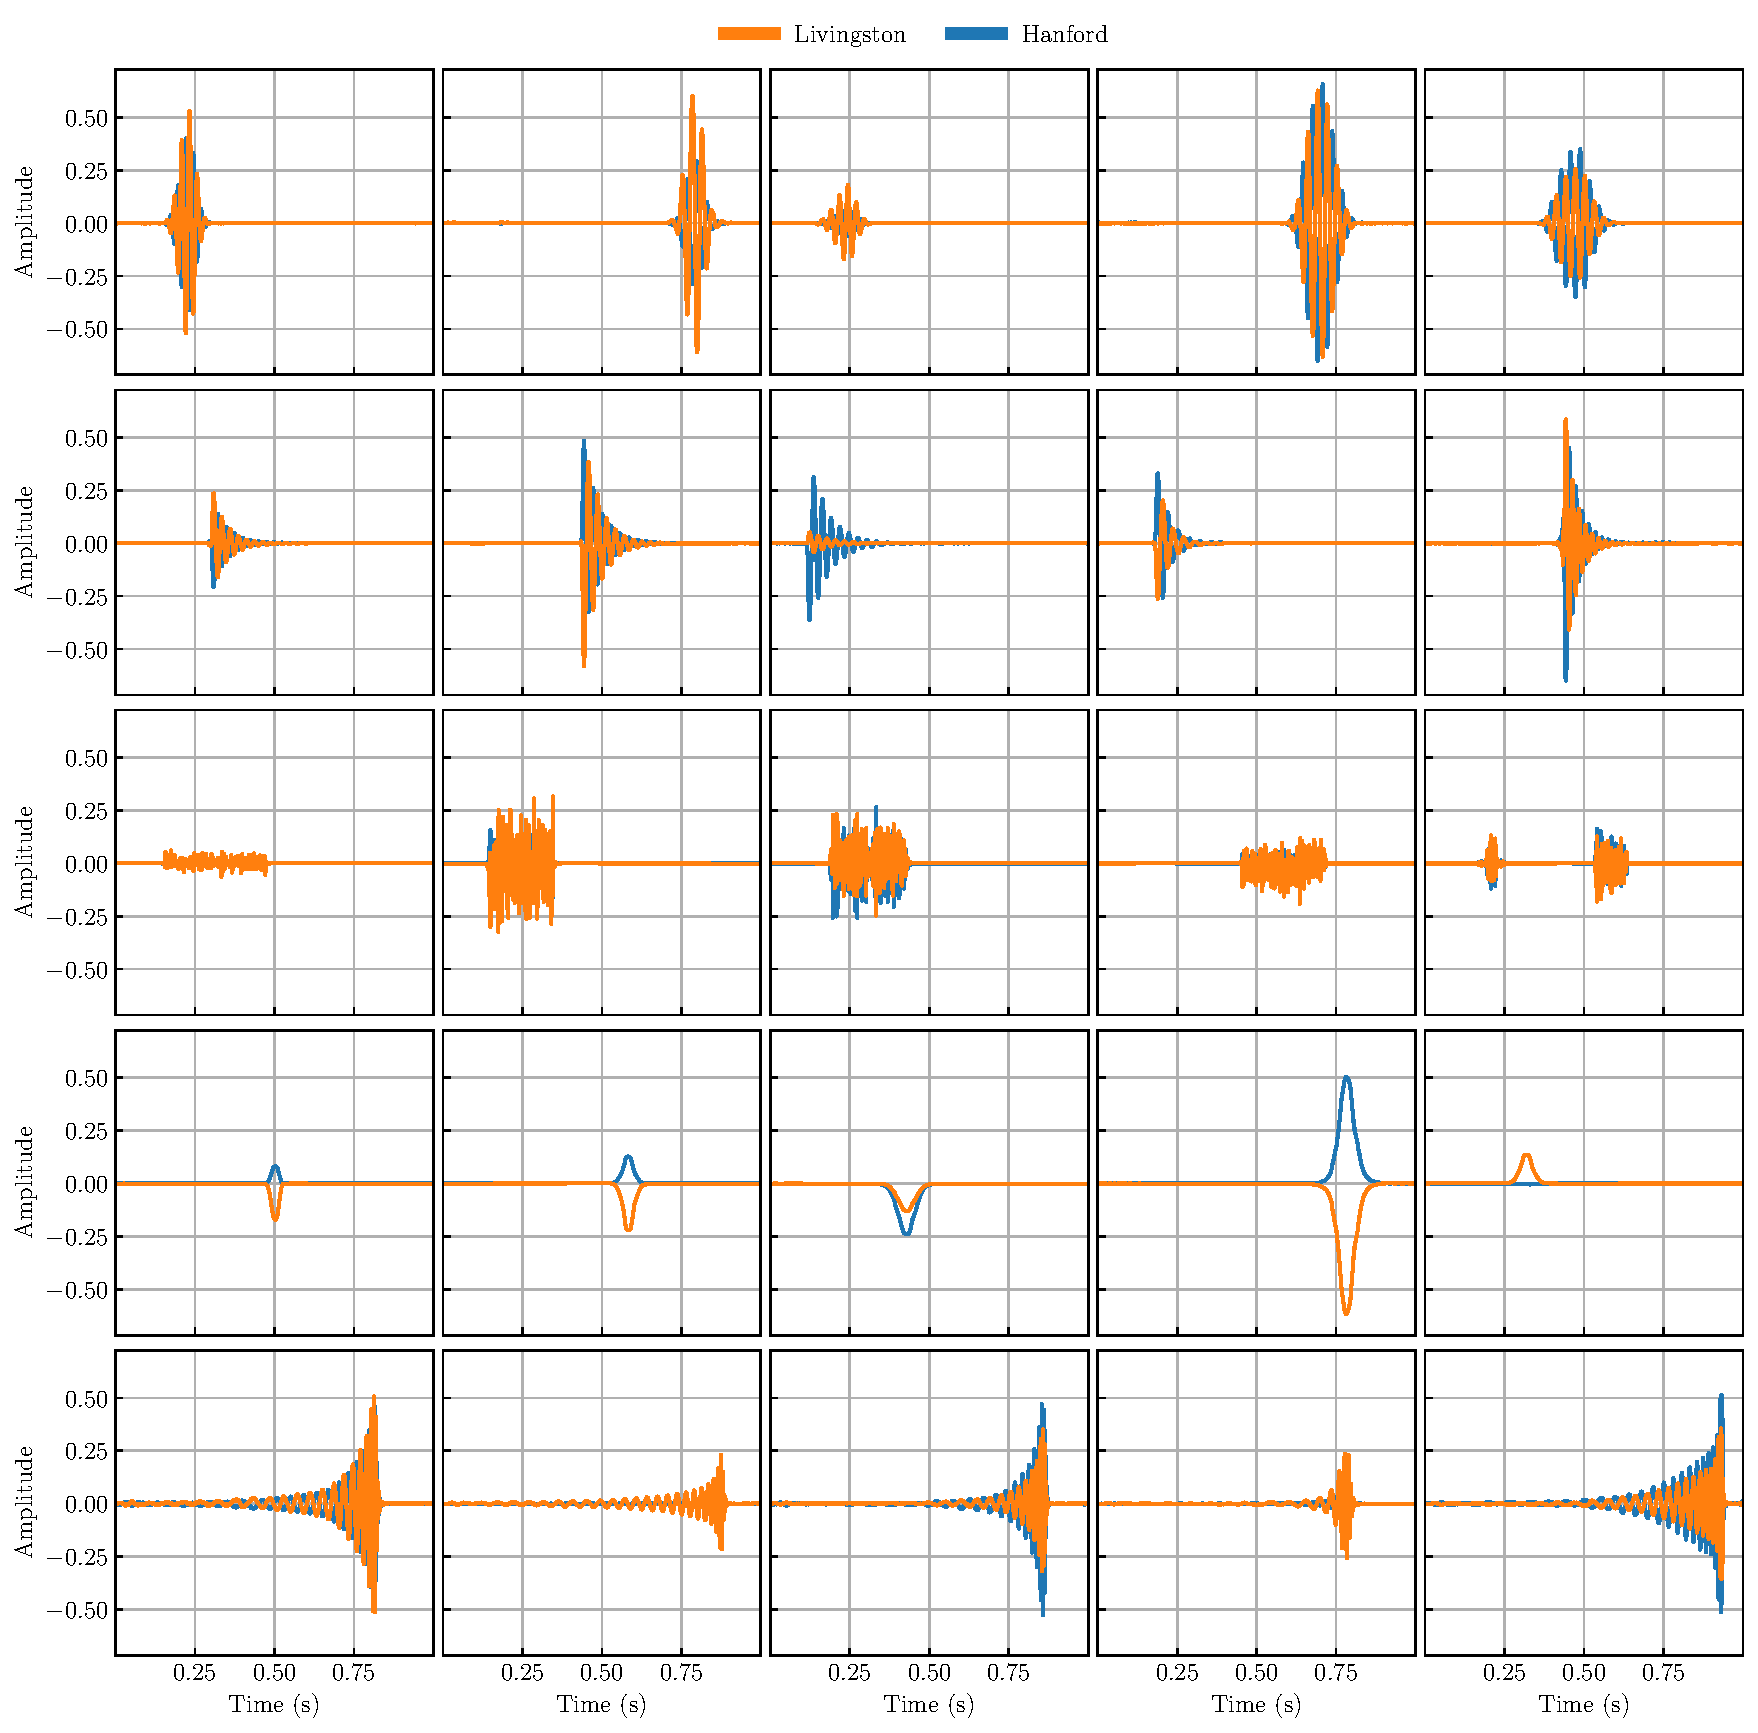
\includegraphics[width=\textwidth]{figures/conditional_gens.pdf}
    \caption{Generated waveforms after training and conditioning on five classes. The generator will output two waveforms as seen by detectors in Hanford (red) and Livingston (blue). The generator is able to capture the characteristics of each waveform and structure the class space to give control over which waveform to generate. Each row shows a random assortment of one of the five classes the GAN is trained on. }
    \label{fig:gen_signals}
\end{figure}

\subsection{Interpolation}
Machine learning algorithms are often described as universal function approximators. In the generators case it maps samples drawn from a 100 dimensional Gaussian space to its representation of the training set. As with any function, there should be a one to one mapping from the domain and co-domain to allow for smooth transitions across the latent space. One advantage of using GANs as a waveform generator is that once it is trained, it can perform rapid generations faster than more intricate and computationally expensive algorithms. For complicated data sets, the network architecture must be diverse and dense enough to capture distinct variations from the training set. Most GANs perform well on relatively low resolution image generations, however, higher resolutions demand larger networks and long training times. GANs attempting to replicate complicated structures and do not have the necessary architecture either struggle to produce results at all or fall into the common failure mode know as mode collapse; where the generator produces a small variety of samples or simply memorises the training set. To test this, we perform linear interpolations in the latent and class space. 

\subsection{Latent space interpolation}
In this section we explore the latent space formed by the generator by interpolation. We take two random points in the latent space and linearly interpolate between them (six times inclusive). These new latent space vectors can now be fed into the generator to make predictions on while keeping the class vectors constant. The third input, the response values are kept constant for each class. The full effect shown in Figure \ref{fig:z_interp}. We can see that each plot shows plausible waveforms suggesting that the generator has constructed a smooth space unlike the discrete training case. Additionally as each class is given the same latent points to interpolate over, we can see that the waveforms cluster together with respect to their parameters. Visually, the sine-gaussian and ring-down waveforms share similar frequencies and the other signals show similar decays and starting epochs. The only exception is BBH waveforms, which is expected as they were trained with more variety of parameters and consistently have their peaks in the last quarter of the time series.

\begin{figure}[ht]
    \centering
    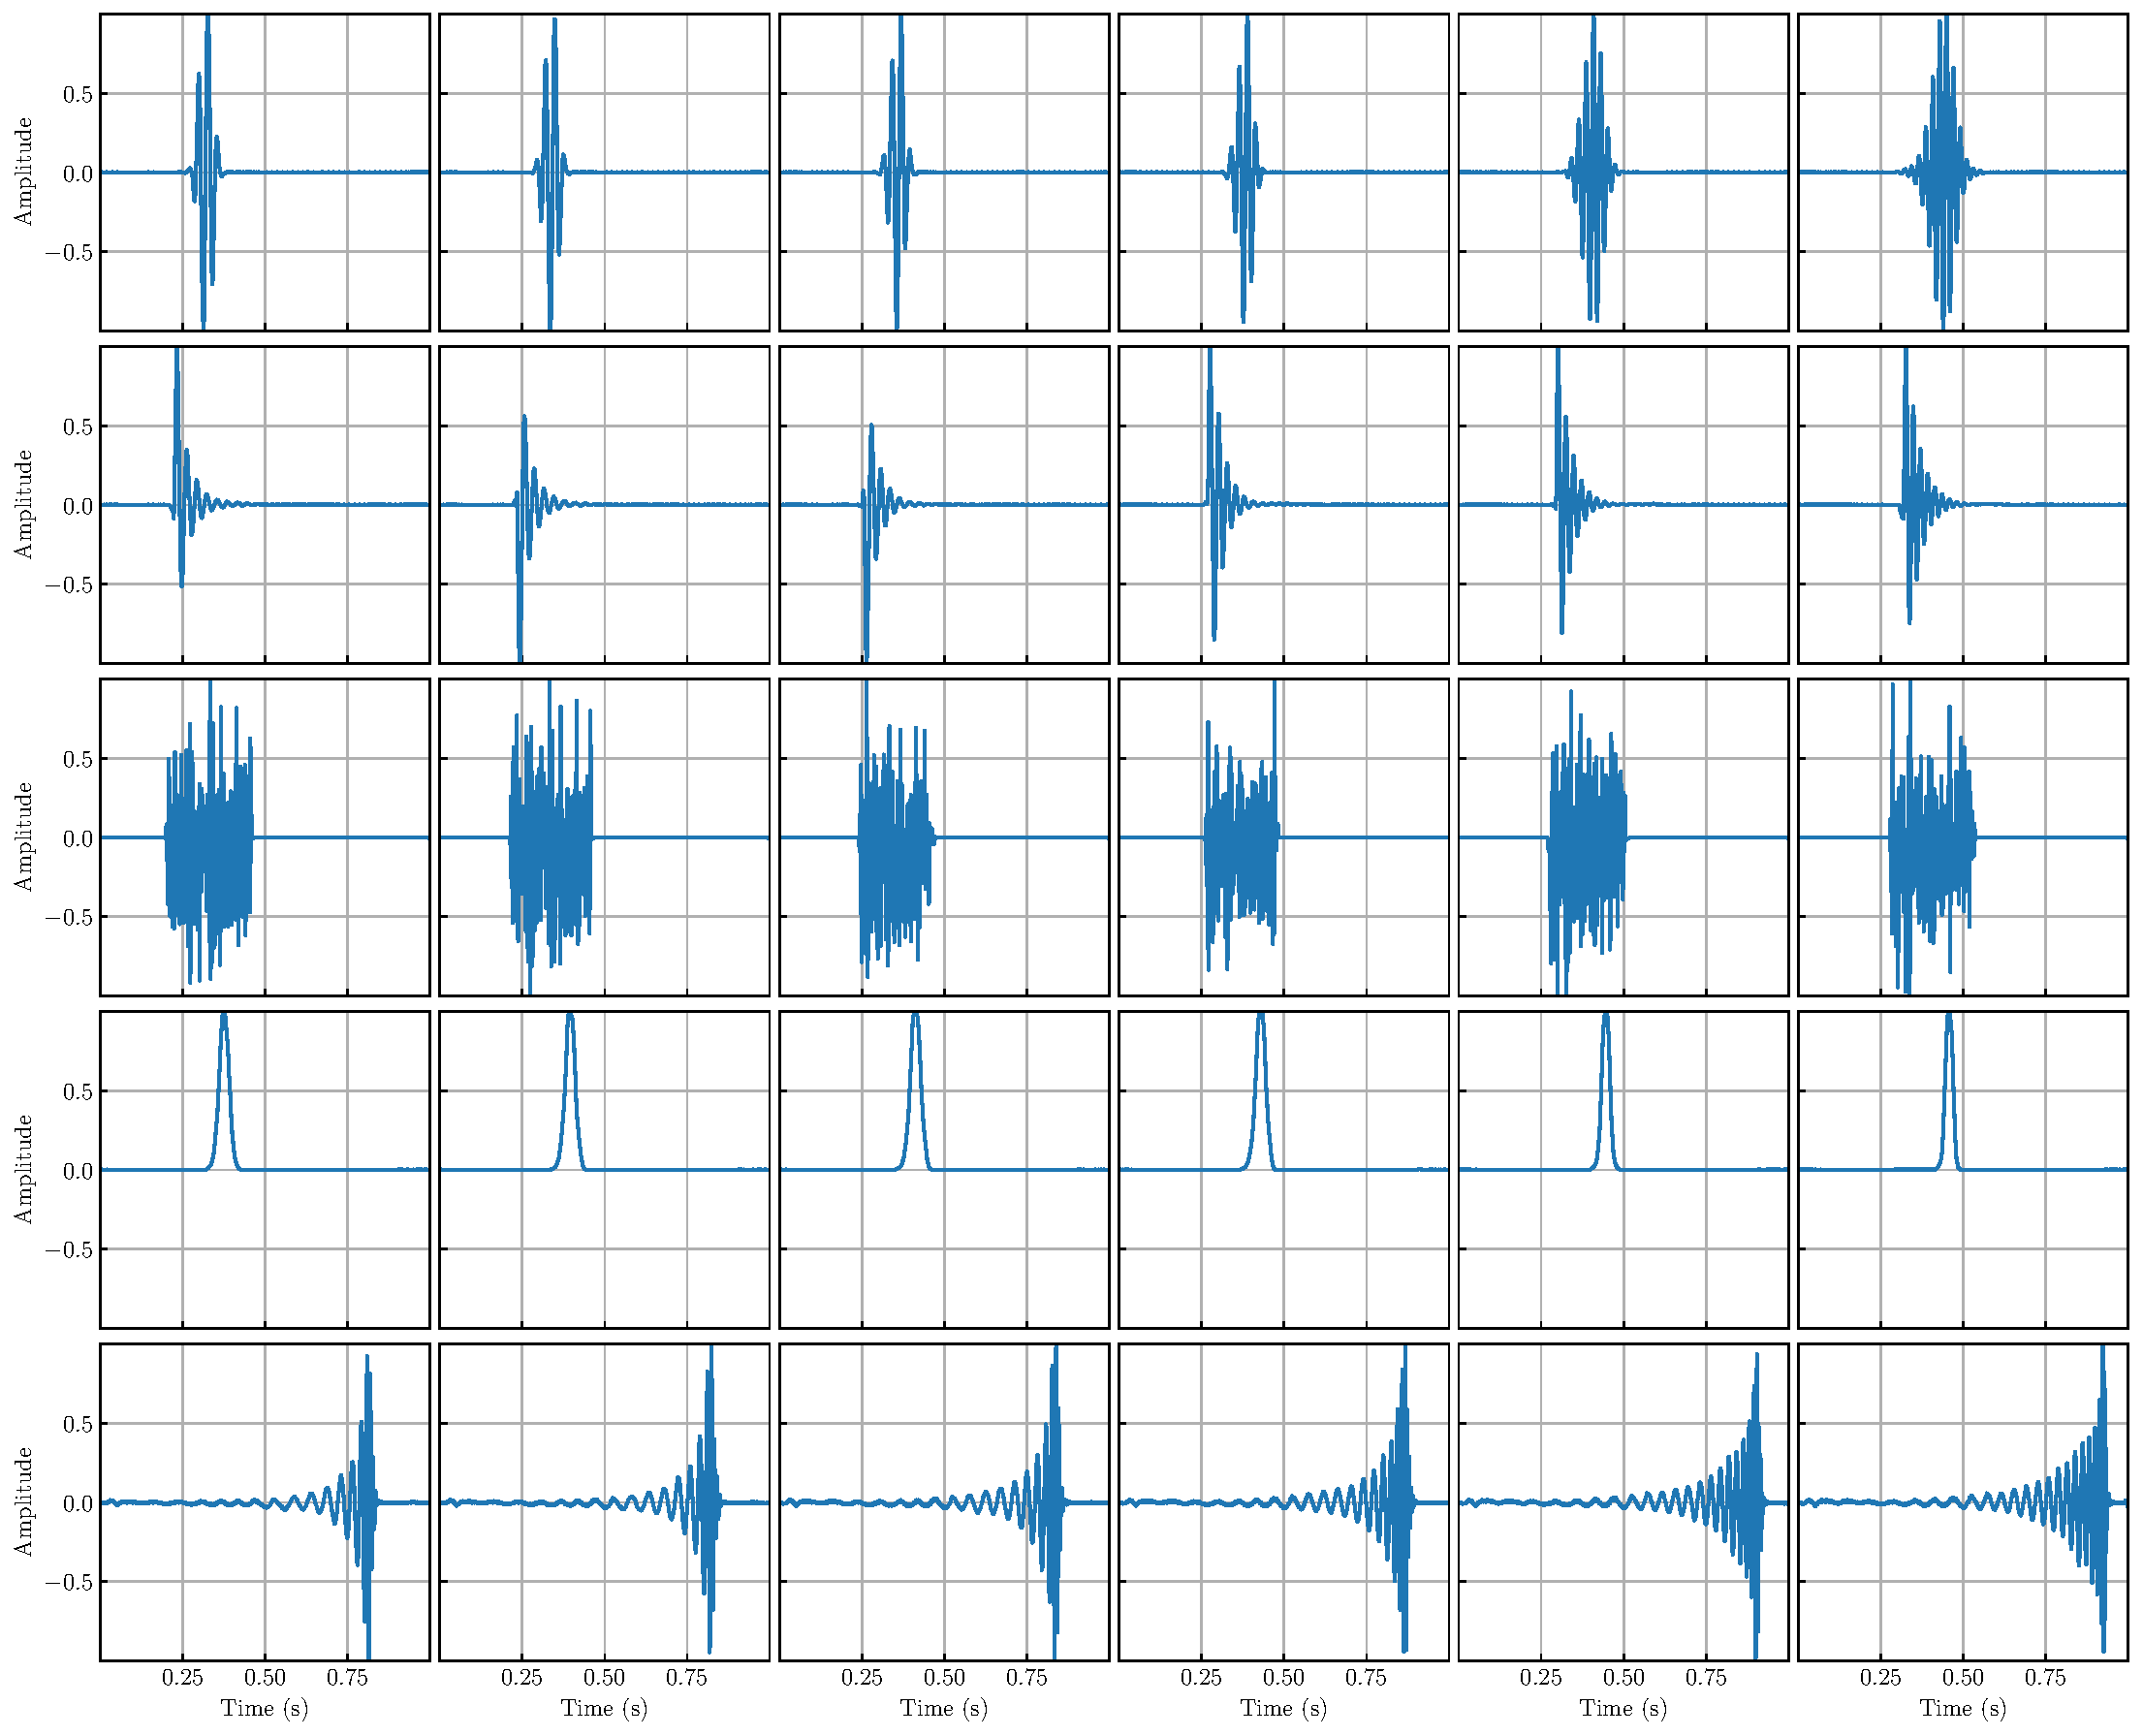
\includegraphics[width=\textwidth]{figures/z_interp_fix_c.pdf}
    \caption{Interpolations between two random latent points in z. Each row uniformly interpolates between two points in $\mathbf{z}$ keeping the class fixed. Only a single waveform from the generator is plotted and each signal is re-scaled to [-1,1] effectively removing the antenna responses for clarity.}
    \label{fig:z_interp}
\end{figure}

\subsection{Class space interpolation}
In order to explore the class space we keep the latent vector held constant and interpolate through the 5 classes. We construct a path between the 5 waveforms and show that the space is populated enough to allow for transitions between classes. Sine-Gaussian to ringdown performs well in interpolation with each signal being a plausible burst GW. It is obvious that the embedding layer has clustered these two groups during training as they share many characteristics. The other signals have sharper transitions but still retain plausible looking waveforms.  

\begin{figure}
    \centering
    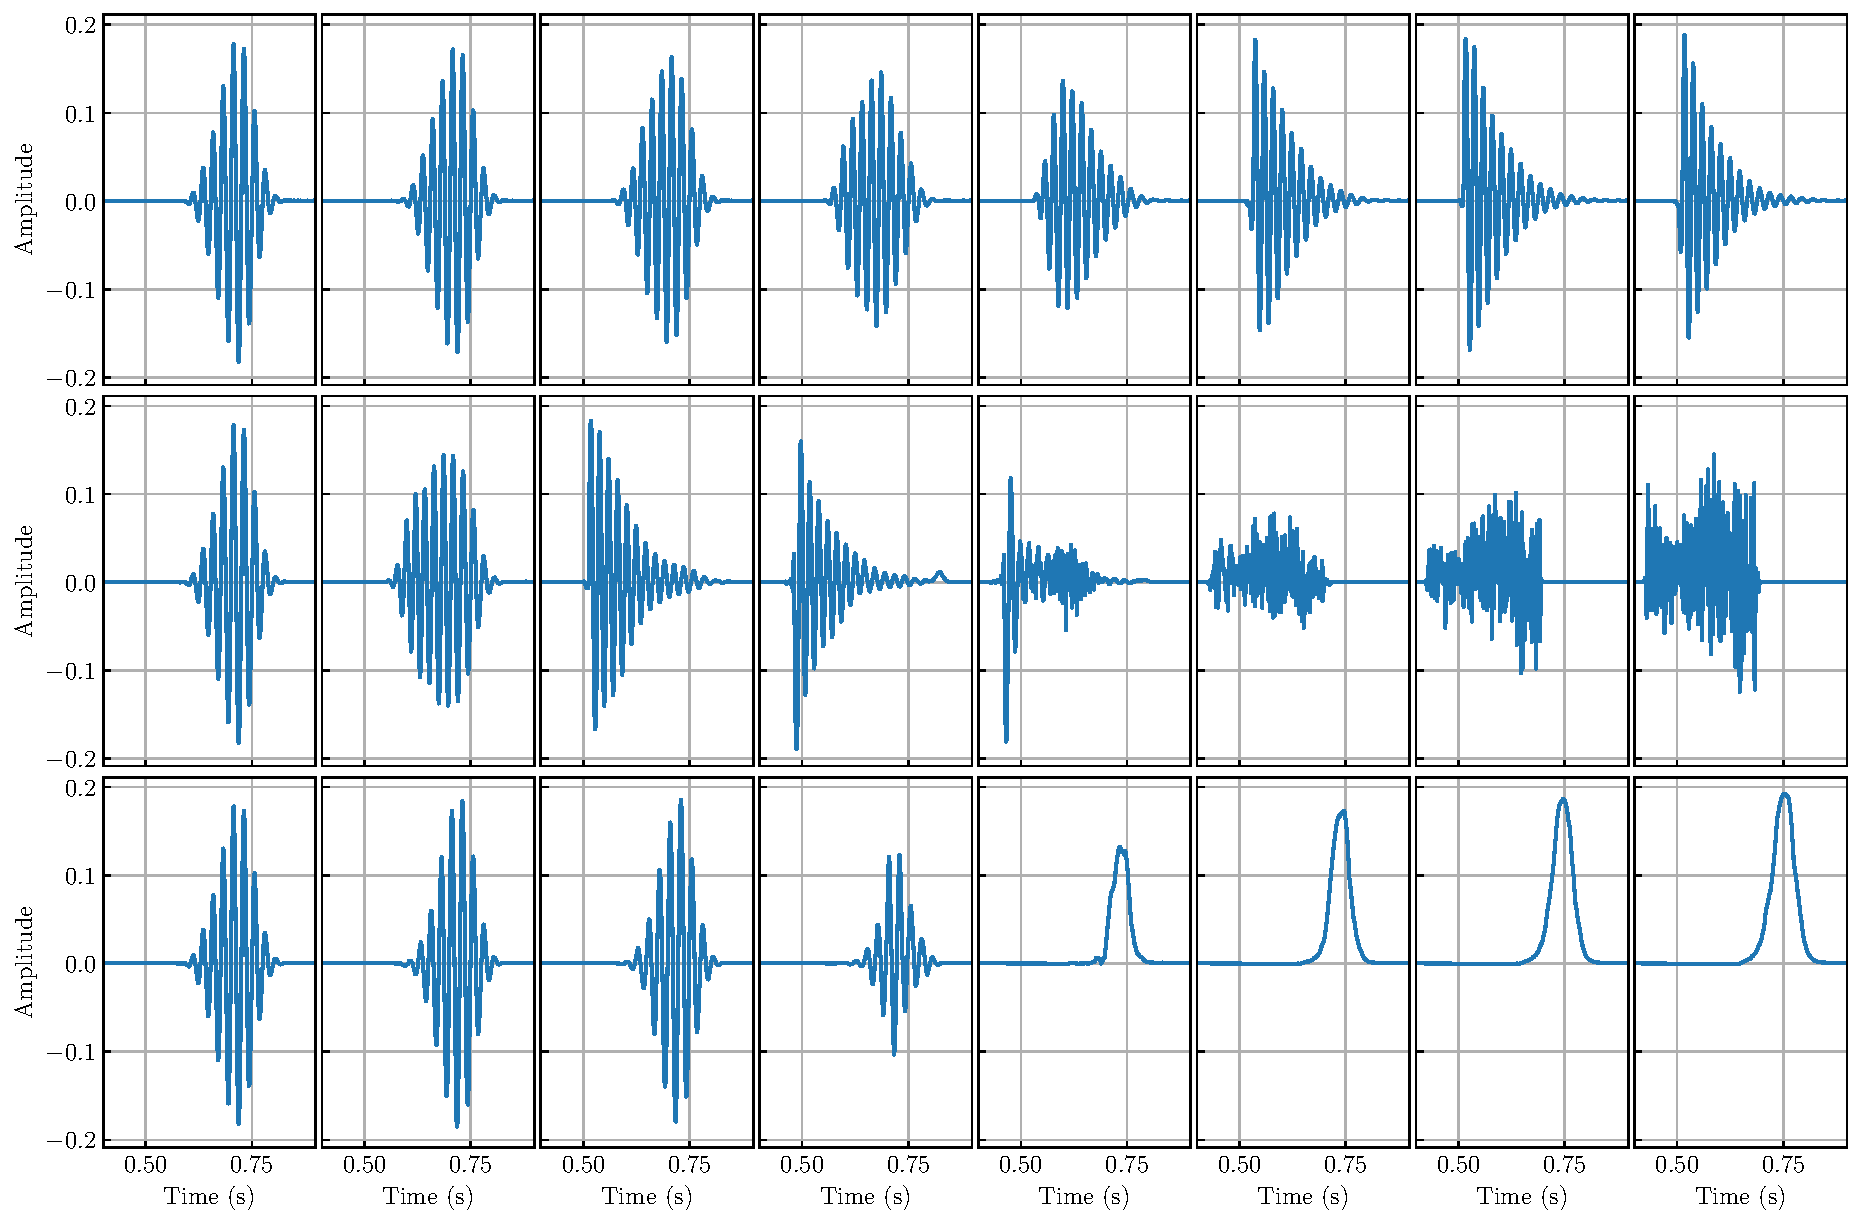
\includegraphics[width=\textwidth]{figures/4_c_interp.pdf}
    \caption{Class space interpolation with latent space held constant throughout. The plots show a zoomed in section of the 1s time interval. Top row: Sine-Gaussian class to ringdown class, Middle Row: Sine-Gaussian class to whitenoise burst class, Bottom row: Sine-Gaussian class to Gaussian class.}
    \label{fig:c_interp}
\end{figure}

\begin{figure}
    \centering
    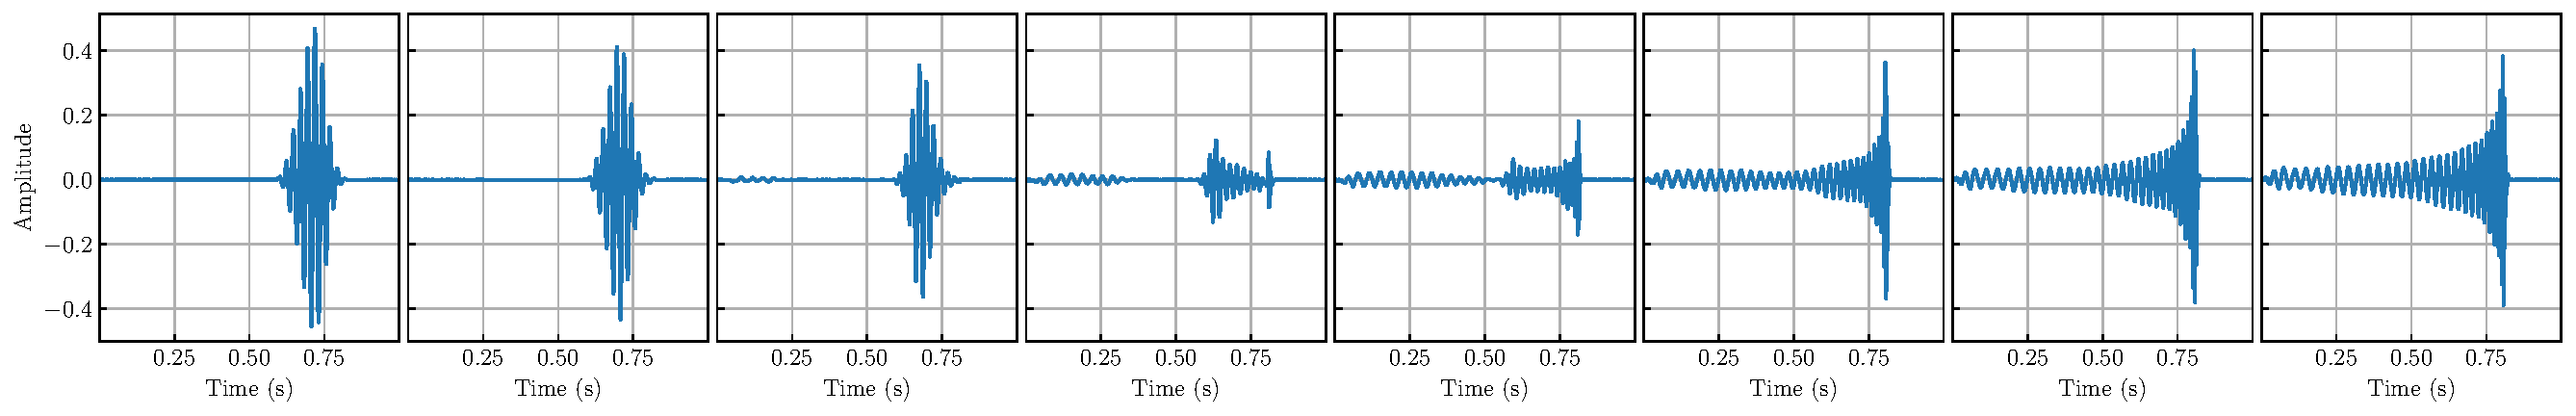
\includegraphics[width=\textwidth]{figures/sg_bbh_interp.pdf}
    \caption{Class space interpolation with latent space held constant throughout. The full 1s interval is plotted for class based interpolations between a Sine-Gaussian and a BBH in spiral.}
    \label{fig:sgbbh_interp}
\end{figure}

\begin{comment}
\begin{figure}
    \centering
    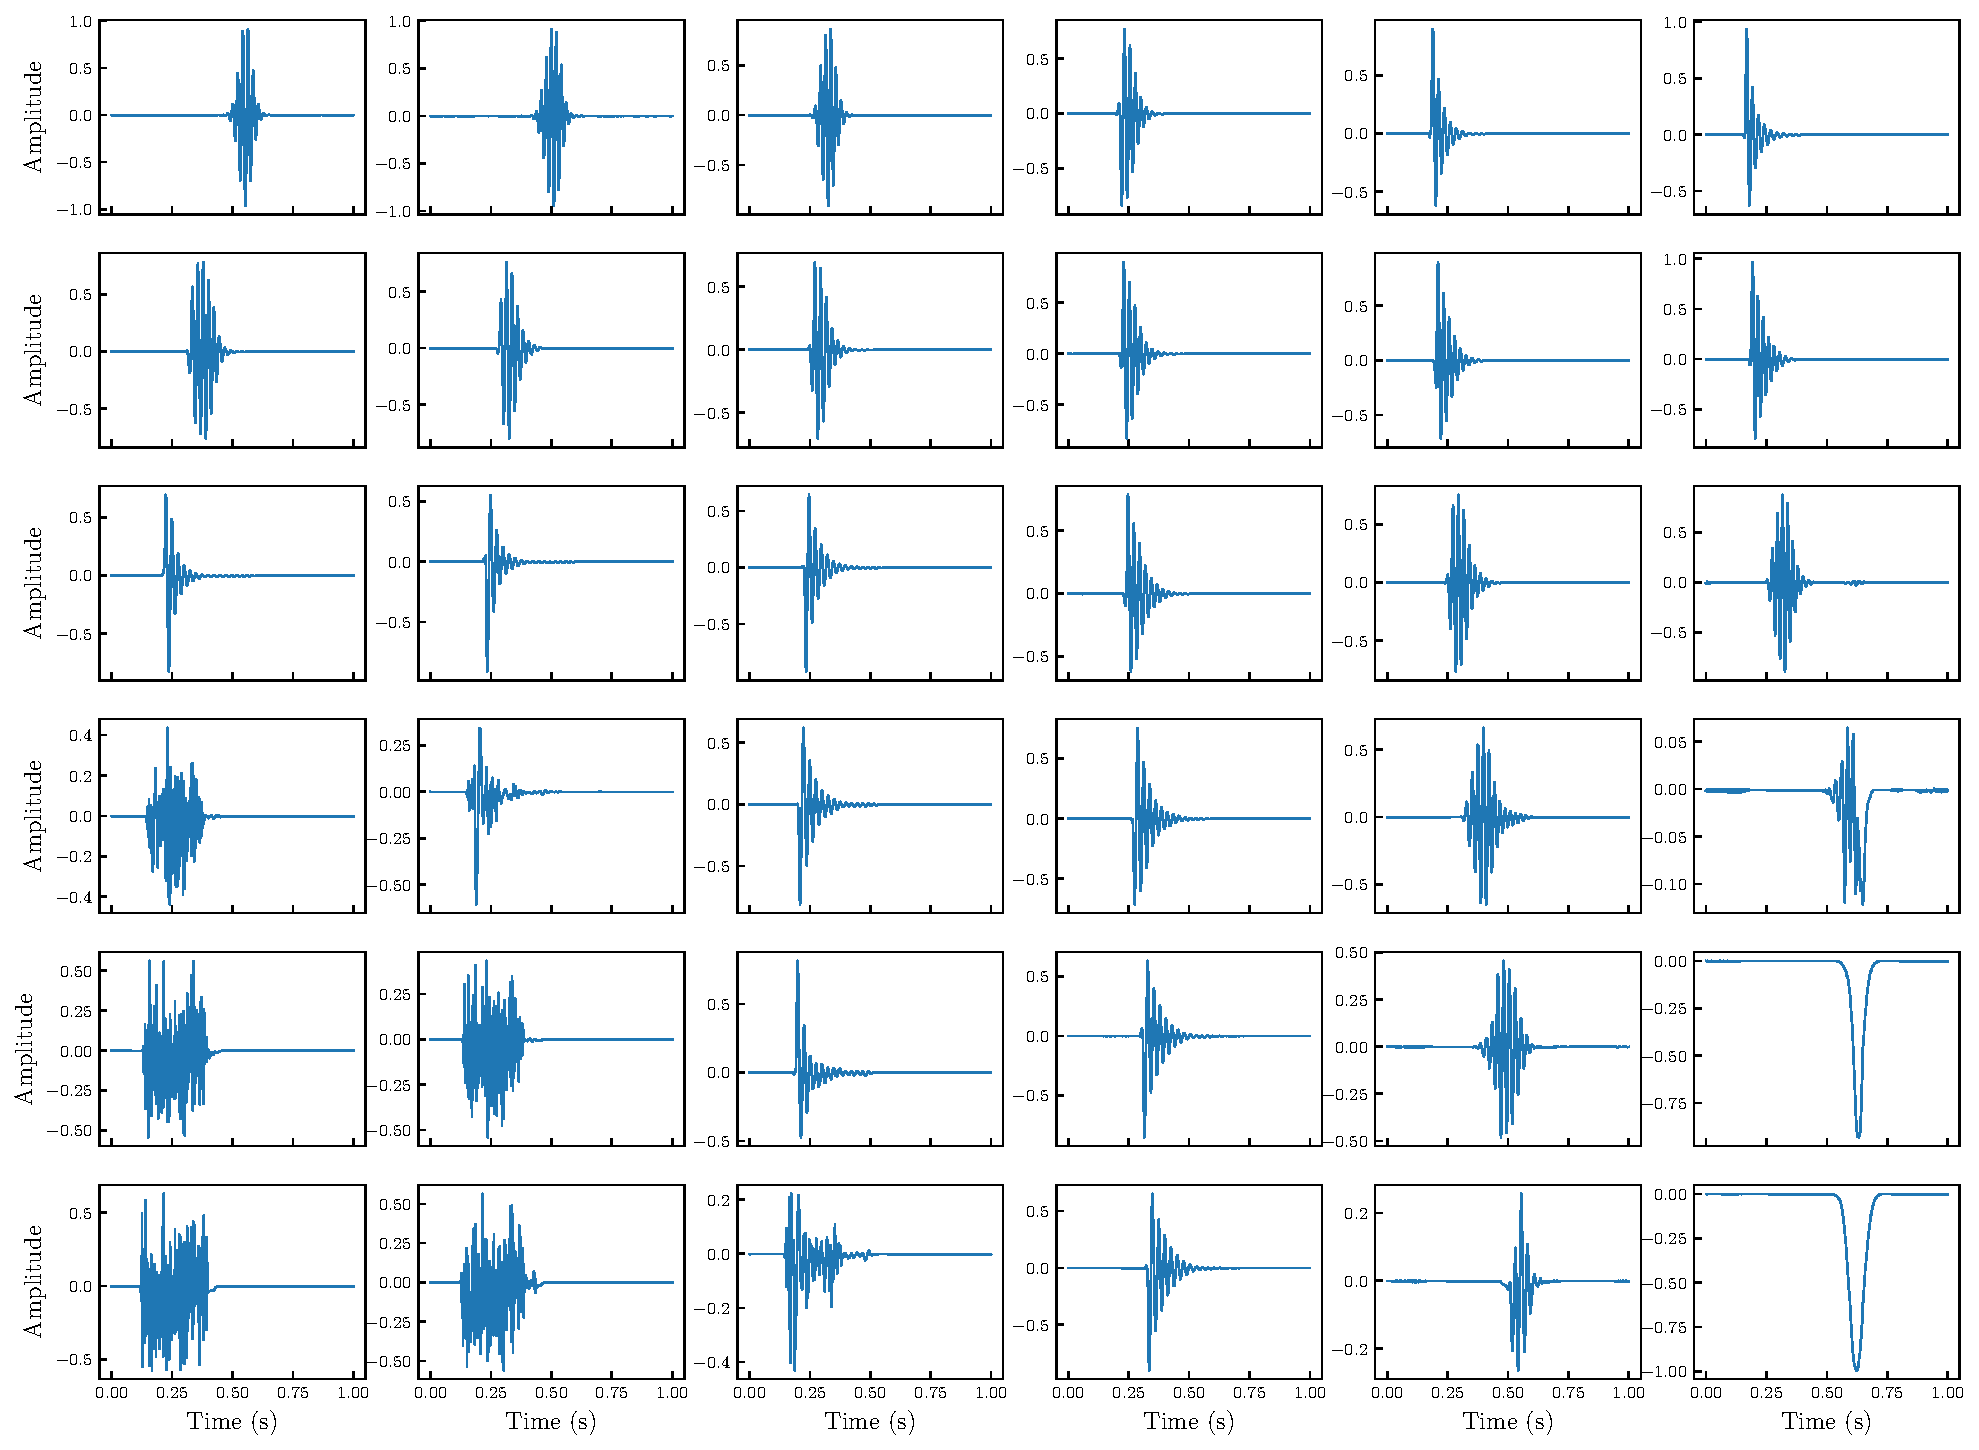
\includegraphics[width=\textwidth]{figures/4_corners.pdf}
    \caption{We generate the four corners of the grid, then interpolate between both the z and c vectors. Although the network was only trained on binary attributes for c, interpolation results show that the computed latent space is smooth between attributes, and not simply discrete to those shown in the training set.}
    \label{fig:4_c_interp}
\end{figure}
\end{comment}

\subsection{Vector Arithmetic}
In DCGANs the authors demonstrated unsupervised vector arithmetic with celebrity face generation. They kept points in the latent space and performed simple vector arithmetic to generate new images. This allows for intuitive and targeted generation of images. However, the authors realised that single images vectors were unstable and there was a need to average three vectors before any arithmetic. DCGANs is unconditional, therefore, the vectors used were chosen empirically, generating many faces and choosing the attributes for study. Here, we show that this GAN only needs a single vector representation and due to conditioning we can have more control over which vectors to use in the arithmetic. In Figure \ref{fig:arithmetic} we generate a whitenoise burst and a BBH insprial using their respective class labels and use a randomised latent point and response. Keeping the latent point and response, we average the two class vectors and use this as input to the generator. Figure \ref{fig:arithmetic} (c) shows the generation based on the combined class vectors which visually looks similar to a supernova waveform. Supernova waveform generations require expensive numerical relativity simulations and various assumptions about the collapse of its parent star. Here, we are able to produce similar waves at a fraction of the expense and we are able to further modify the resultant by using different latent space samples. \jordan{this is the adding noise thing but i need to work out the correct way to do it with the directional vector}. 

\begin{figure}
  \centering
  \begin{tabular}[b]{c}
    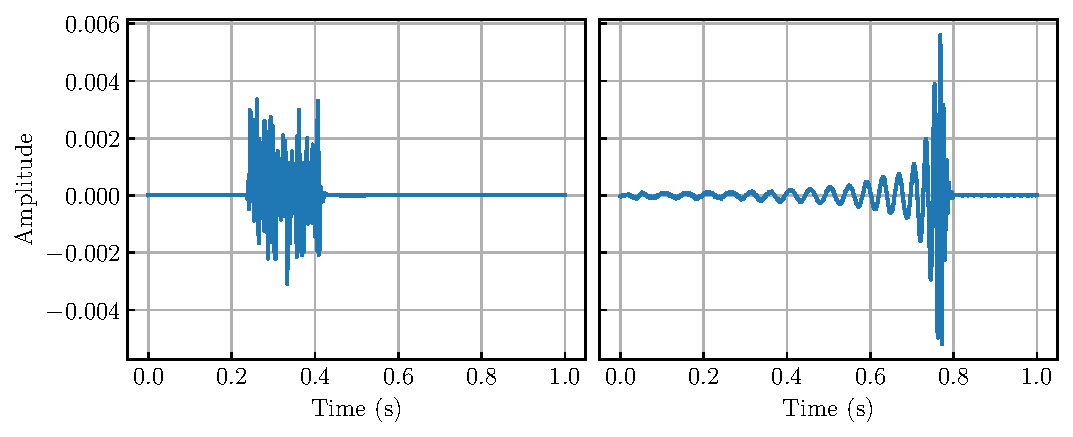
\includegraphics[width=0.9\textwidth]{figures/wn+bbh.pdf} \\
    \small ~~~~~~~~~(a)
  \end{tabular} %\qquad
  
  \begin{tabular}[b]{c}
    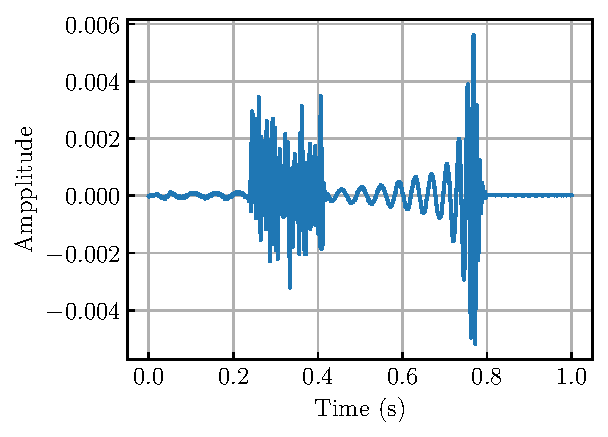
\includegraphics[width=0.46\textwidth]{figures/ambient_result.pdf} \\
    \small ~~~~~~~~(b)
  \end{tabular}
 \begin{tabular}[b]{c}
    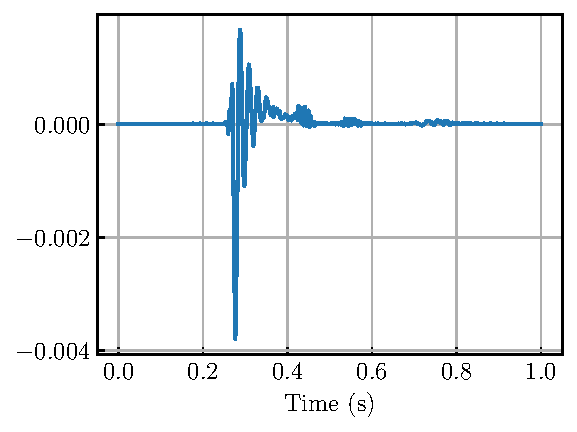
\includegraphics[width=0.44\textwidth]{figures/arithmetic_result.pdf} \\
    \small ~~~~~~~~(c)
  \end{tabular}
  \caption{Conditional vector arithmetic. (a) Generated samples of a whitenoise burst and BBH insprial. (c) Effect of naively adding the components from (a) in the time domain. \jordan{just adding the two signals post generation} (c) Generation from the combined class vectors. }
  \label{fig:arithmetic}
\end{figure}


\begin{comment}
\begin{figure}
    \centering
    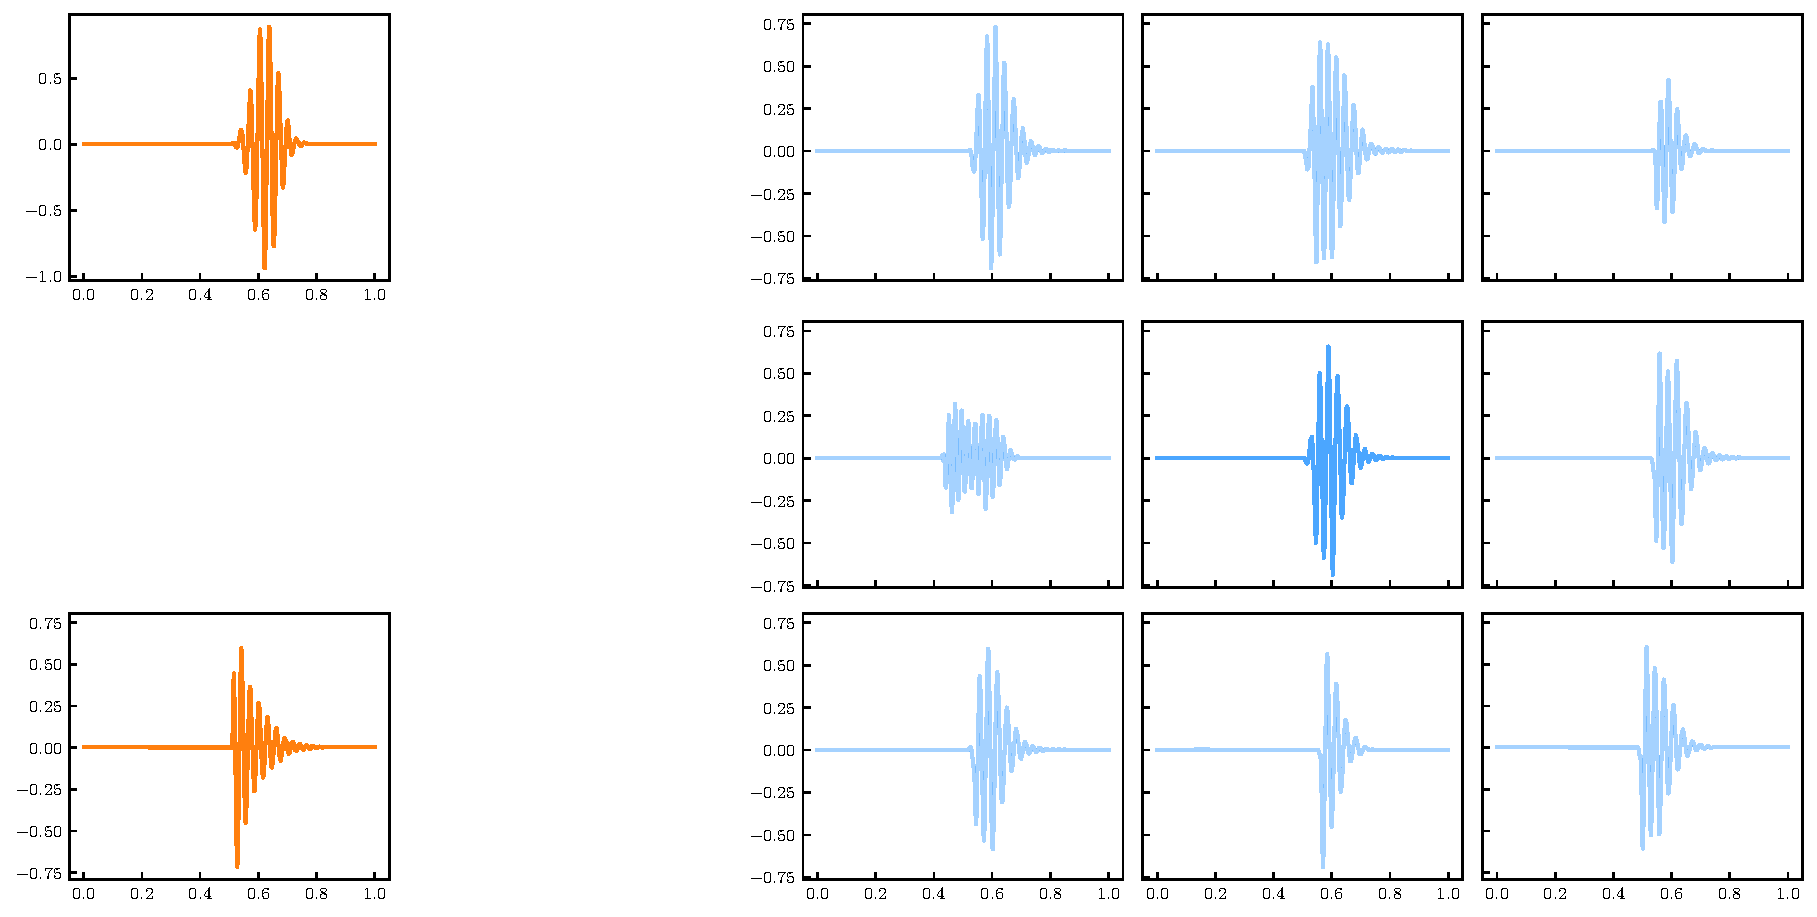
\includegraphics[width=\textwidth]{figures/arithm.pdf}
    \caption{Vector arithmetic for unmodelled waveforms. Keeping the z vectors constant and generating two classes of signals, their class embedding vectors can then be averaged to produce a new class. The generator produces a waveform of this hybrid class (middle of right plot). For the surrounding 8 plots we add a small variance of Gaussian noise to the new class. }
    \label{fig:add}
\end{figure}
\end{comment}
\subsection{Classifier}
\jordan{I'm working on this part and how to present the auxiliary part.}


%%%%%%%%%%%%%%%%%%%%%%%%%%%%%%%%%%%%%%%%%%%%%%%%%%%%%%%%%%%%%%%%%%%%%%%%%%%%%%
\section{Conclusions}
%%%%%%%%%%%%%%%%%%%%%%%%%%%%%%%%%%%%%%%%%%%%%%%%%%%%%%%%%%%%%%%%%%%%%%%%%%%%%%
In this work we present the potential of Generative Adversarial Networks for burst gravitational wave analysis. We have shown that GANs have the ability to generate 5 class varieties of modelled burst \ac{GW} signals that can be generated at whim. The latent and class spaces were explored through interpolation and suggest that the space provides smooth translations between classes and overall waveform shape. We then showed targeted waveform generation by mixing classes to produce new unmodlled waveform varieties that can be used to test current burst search pipelines. \jordan{couple of sentences about classifier}. 

In order to extend this work to a viable burst wave generator and classifier a few points require further research. In principle it is trivial to add another detector inside the response layer \jordan{response is the wrong thing to say since the time delay isnt really a response, extrinsic layer? just non trainable layer? The box?}, however, as this now 3 dimensional signal is feed to the discriminator this will no doubt require further tweaking of the network. We can add more burst-like wave forms in the training set, like detector glitches which would similarly require further network design. The work presented here is noise free. To havea complete generation and detection package we would like to train the network on signals hidden in additive Gaussian noise and test the ability of the auxiliary classifier. 

The approach shown in this work shows promise in generating unmodelled burst waveforms from exotic sources. Having the ability to quickly generate new waveforms is essential to test current detection schemes and their susceptibilty to unmodelled sources. We belive that GANs have the ability to generate high fidelity waveforms at a fraction of the computational expense and do not rely on large prior parameter space. Having banks of these waveforms at hand can aid in our understand of the physics processes behind these non-standard gravitational wave emitters.  

\jordan{I want to include a link to the github etc but also a google collab scrip like the one for BigGANs: \\
\url{https://colab.research.google.com/github/tensorflow/hub/blob/master/examples/colab/biggan_generation_with_tf_hub.ipynb.} 
It's fun and gives a better feel for the interpolating that static images.}

\begin{comment}
\begin{itemize}
\item Summarise the paper
\item Dedicate a paragraph to each of the key results discussed in the previous
section
\item Have at least one paragraph on the future directions of this work
\item Conclude with a positive paragrpah about the potential uses and impact of
the approach.
\end{itemize}
\end{comment}

\section*{References}
\bibliography{iopart-num}

\clearpage

\appendix
\section{List of hyperparameters}
\begin{table}[hb]
\caption{ACGAN architecture}
\footnotesize
\begin{tabular}{@{}lllllll}
\br
 Operation & Kernel & Strides & Output Shape & BN & Dropout & Activation \\
\mr
 G(\textbf{z}): Input \textbf{z} $\sim$ Normal(0,0.02) & N/A & N/A & (100,) & \ding{55} & 0 & N/A \\  
 Dense & N/A & N/A & (32768,) & \ding{55} & 0 & ReLU \\  
 Class input c & N/A & N/A & (1,) & \ding{55} & 0 & N/A \\
 Embedding & N/A & N/A & (1, 120) & \ding{55} & 0 & N/A \\
 Dense & N/A & N/A & (1,128) & \ding{55} & 0 & ReLU \\ 
 Reshape \textbf{z} & N/A & N/A & (128, 256) & \ding{55} & 0 & N/A \\
 Reshape c & N/A & N/A & (128, 1) & \ding{55} & 0 & N/A \\
 Concatenate & N/A & N/A & (128, 257) & \ding{55} & 0 & N/A \\
 Reshape & N/A & N/A & (64, 514) & \ding{55} & 0 & N/A \\
 Transposed Convolution & 18x1 & 2 & (256, 256) & \ding{51} & 0 & ReLU\\
 Transposed Convolution & 18x1 & 2 & (512, 128) & \ding{55} & 0 & ReLU\\
 Transposed Convolution & 18x1 & 2 & (1024, 64) & \ding{55} & 0 & ReLU\\
 Convolution & 18x1 & 1 & (1024, 1) & \ding{55} & 0 & Tanh \\
 Sky input & N/A & N/A & (3,) & \ding{55} & 0 & N/A \\
 Concatenate & N/A & N/A & (1027,) &  \ding{55} & 0 & N/A \\
 Lambda & N/A & N/A & (1024, 2) & \ding{55} & 0 & N/A \\
 D(\textbf{x}): Input \textbf{x} & N/A & N/A & (1024, 2) & \ding{55} & 0 & N/A \\
 Convolution & 14x1 & 2 & (512, 64) & \ding{55} & 0.5 & Leaky ReLU \\
 Convolution & 14x1 & 2 & (256, 128) & \ding{55} & 0.5 & Leaky ReLU \\
 Convolution & 14x1 & 2 & (128, 256) & \ding{55} & 0.5 & Leaky ReLU \\
 Convolution & 14x1 & 2 & (64, 512) & \ding{55} & 0.5 & Leaky ReLU \\
 Flatten & N/A & N/A & (32768,) & \ding{55} & 0 & N/A \\
 Dense & N/A & N/A & (1,) & \ding{55} & 0 & Sigmoid \\
 Dense & N/A & N/A & (5,) & \ding{55} & 0 & Softmax \\
\br
 Optimizer & \multicolumn{6}{l}{Adam($\alpha$ = 0.0002, $\beta_{1}$ = 0.5)} \\
 Batch size & \multicolumn{6}{l}{128}  \\
 Iterations & \multicolumn{6}{l}{60000}  \\
 Leaky ReLU slope & \multicolumn{6}{l}{0.2} \\
 Weight initialization & \multicolumn{6}{l}{Gaussian($\mu$ = 0, $\sigma$ = 0.02)} \\
 Generator loss & \multicolumn{6}{l}{Binary cross-entropy} \\
 Discriminator loss & \multicolumn{6}{l}{Binary cross-entropy \& sparse categorical cross-entropy} \\ 
 \br
\end{tabular}\\
\label{Tab:hyperparameters}
\end{table}
\normalsize

\section{Many more generated examples}

\end{document}

